\documentclass{beamer}

\usepackage[T1]{fontenc}
\usepackage[utf8]{inputenc}
\usepackage{lmodern}
\usepackage{graphicx}
\usepackage[absolute,overlay]{textpos}
\usepackage{multicol}
\usepackage{listings}
\usepackage{svg}

%% Beamer customization--------------------------------------------------------

\usepackage{xcolor}


\usepackage{tikz}

\usetheme{Warsaw}

%% Themes
% Outer themes
\useoutertheme{shadow}
% Rounded boxes and shadows
\useinnertheme[shadow=true]{rounded}
% Solid \item symbols
\useinnertheme{circles}

%% Custom colors
\definecolor{rltgreen}{rgb}{0,0.5,0}
\definecolor{pasteur}{RGB}{0,90,154}
\setbeamerfont{block title}{size={}}
\setbeamercolor{structure}{fg=pasteur}
\setbeamercolor{item}{fg=pasteur}


%Color of title
\setbeamertemplate{frametitle}
{    \nointerlineskip
    \begin{beamercolorbox}[sep=0.3cm,ht=1.8em,wd=\paperwidth]{frametitle}
        \vbox{}\vskip-2ex%
        \strut\insertframetitle\strut
        \vskip-0.8ex%
    \end{beamercolorbox}
}
% Hide navigation symbols
\setbeamertemplate{navigation symbols}{}

%% Title block
\setbeamercolor*{title}{use=structure,fg=white,bg=pasteur}



\makeatletter

%% Top infolines
\setbeamertemplate{headline}{%
\leavevmode%
  \hbox{%
%    \begin{beamercolorbox}[wd=\paperwidth,ht=2.5ex,dp=1.125ex]{palette quaternary}%
%    \insertsectionnavigationhorizontal{\paperwidth}{}{\hskip0pt plus1filll}
%    \end{beamercolorbox}%
  }
}


%% Define Snakemake -----------------------------------------------------------

\definecolor{eclipseBlue}{RGB}{42,0.0,255}
\definecolor{eclipseGreen}{RGB}{63,127,95}
\definecolor{eclipsePurple}{RGB}{127,0,85}

\lstset{language=Python}
\lstset{
    basicstyle=\scriptsize\ttfamily,
    morekeywords={rule, output, shell, params, run, configfile, temp, log},
    showstringspaces=false,
    commentstyle=\color{eclipseGreen}, % style of comments
    keywordstyle=\color{eclipsePurple}, % style of keywords
    stringstyle=\color{eclipseBlue}, % style of strings
}



%% Set up title ---------------------------------------------------------------

\title[SequanaCoverage]{Characterization of Genome Coverage and Identification 
of Genomic Regions of Interest (ROIs)}

\author[D.Desvillechabrol \& T.Cokelaer]{Dimitri Desvillechabrol and Thomas Cokelaer}

\date{September 25th 2017, Institut Curie, Paris}


\AtBeginSection[]{
  \begin{frame}
  \vfill
  \centering
  \begin{beamercolorbox}[sep=8pt,center,shadow=true,rounded=true]{title}
    \usebeamerfont{title}\insertsectionhead\par%
  \end{beamercolorbox}
  \vfill
  \end{frame}
}


\begin{document}
%% Title slide -------------------------------------------------------------
\begin{frame}[plain]
    \titlepage
    \begin{textblock*}{5cm}(8cm,0.3cm)
        
\includegraphics[scale=0.09]{../../images/Institut_Pasteur.png}   
    \end{textblock*}
\end{frame}

%% Slides ---------------------------------------------------------------------

\begin{frame}
\frametitle{Genome coverage}

\textbf{Definition:} The number of reads mapped to a specific position, $b$, 
within the reference genome. \\
\vspace{1em}
\textbf{Notation:} $ C(b)$ also denoted $C_b$\\
\vspace{1em}
\textbf{Theoretical distribution:} Poisson distribution but in practice over 
dispersed. The poisson parameter is distributed according to a Gamma hence 
leading to a negative binomial (See e.g., Linder et al 2013).
\end{frame}


\begin{frame}
\frametitle{\small Bacteria case (low/high $\mu$ components and del. region)}
\begin{center}
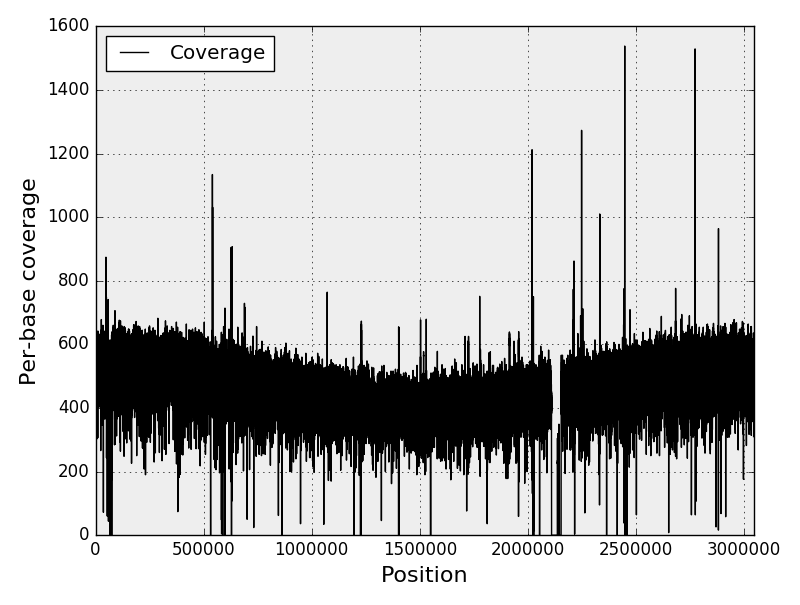
\includegraphics[height=0.9\textheight, width=1\textwidth]{images/coverage_bacteria.png}
%Problems (see next figures)
%   Low and high frequency trends prevent fitting of any distribution
%    Some regions are deleted.
%    Others are repeated or over covered by several folds
\end{center}
\end{frame}

\begin{frame}
\frametitle{\small Virus case}
\begin{center}
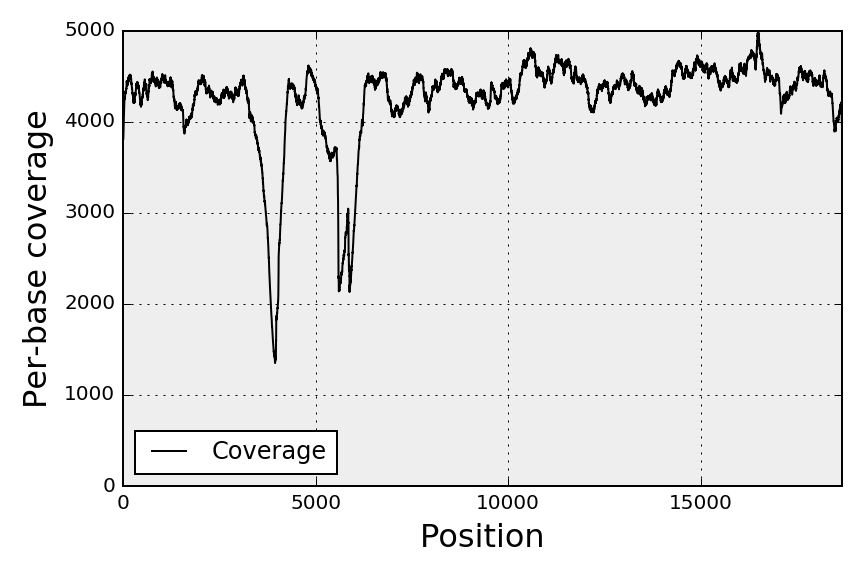
\includegraphics[height=0.9\textheight, width=1\textwidth]{images/coverage_virus.png}
%Problems (see next figures)
%   Low and high frequency trends prevent fitting of any distribution
%    Some regions are deleted.
%    Others are repeated or over covered by several folds
\end{center}
\end{frame}


\section{
Question: how to automatically detect and characterise under and 
over covered genomic regions}



\begin{frame}{The algorithm}
  \begin{enumerate}
    \item Detrending (running median)
    \item Mixture model estimation (Gaussian approximation)
    \item Set a statistics (z-score)
    \item Clustering (double threshold)
  \end{enumerate}
\end{frame}


%%%%%%%%%%%%%%%%%%%%%%%%%%%%%%%%%%%%%%%%%%%%%%%%%%%%%%%%%%%%%%%%%%%%%%%%%%
\begin{frame}
\frametitle{1. Detrending}
 
We divide $C_b$ by its moving average (MA), or even better its 
running median (RM) defined as 

\begin{equation}
RM_W(b) = \textrm{median}\left({C(b-V), \dots , C(b+V)}\right) \nonumber
\end{equation}

$W$ is the running window and $V=(W-1)/2$.

\begin{block}{The normalised genome coverage}
\begin{equation}
\widetilde{C}_b = \frac{C_b}{RM_W(b)}  \nonumber
\end{equation}
\end{block}

\pause

\begin{block}{Computational note}
Running median is slow due to the sorting task. \\
\textbf{Solution:} a rolling window + a bisection method to insert 
new element in a sorted list + efficient insert/deletion in a 
list (B-tree) helps:  \textbf{Only a few seconds to scan a 3Mb-length genome.}
\end{block} 
\end{frame}


\begin{frame}
\frametitle{Normalised coverage}
\begin{center}
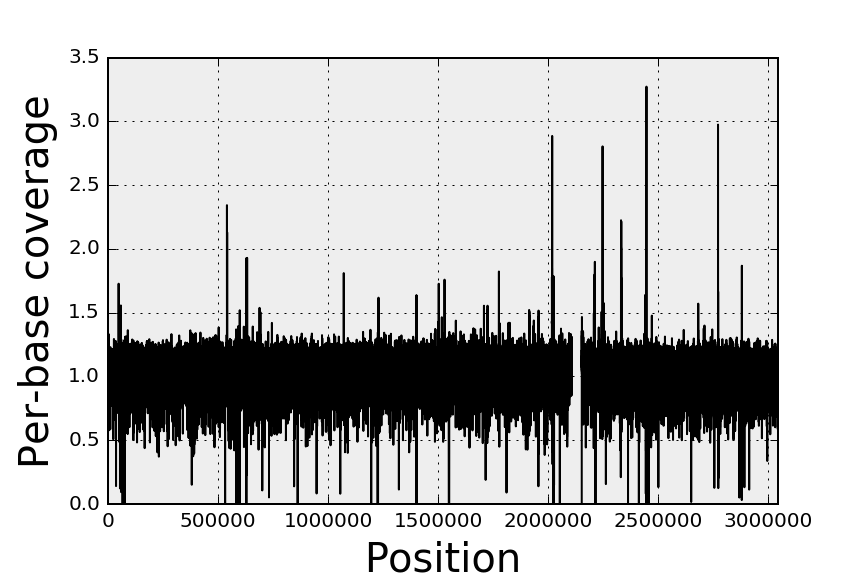
\includegraphics[height=0.9\textheight, 
    width=1\textwidth]{images/coverage_normalised.png}
\end{center} 
\end{frame}


\begin{frame}
 \frametitle{2. Building a statistics}
 
\textbf{Definition:} the normalised data can be decomposed 
into a \textbf{\textcolor{blue}{central}}
distribution $\widetilde{C}^0$ and a set 
of \textbf{\textcolor{blue}{outliers}} $\widetilde{C}^1$ (above and below 
the central distribution)

\begin{equation} 
\widetilde{C}_b  = \left\{ \widetilde{C}^0_b, \{\widetilde{C}^+_b, \widetilde{C}^-_b\}  \right\}
\nonumber
\end{equation}
\vspace{1cm}
\textbf{Hypothesis 1:} Central distribution is predominant.
\begin{equation}
\left|\widetilde{C}^0_b\right| > \left|\widetilde{C}^1_b\right| \nonumber
\end{equation}
\end{frame}



\begin{frame}
\textbf{Hypothesis 2:} The normalised genome coverage follows a 
Gaussian distribution in particular the central distribution

\begin{equation}
PDF(\widetilde{C}_b^0) \sim \mathcal{N}(\mu_0, \sigma_0) \nonumber
\end{equation}

We consider regime with $\delta \gg 1$. However, the algorithm 
works for low values: $\delta \sim 5-10$.
 \end{frame}


\begin{frame}
 
The central distribution $C_0$ will be fitted to a Gaussian 
distribution while the outliers will be fitted to another 
distribution.

\begin{itemize}
\item With an EM algorithm using $k=2$ distributions we can estimate the parameters. 
\item The parameters of the \textcolor{blue}{outliers} components are not used. 
\item The average of the \textcolor{blue}{central} distribution is  1 (by definition)
\item Note that the average of the \textcolor{blue}{outliers} can be around 1 as
well if the weights of C+ and C- are equivalent
\end{itemize}
\end{frame}


\begin{frame}
\frametitle{}
\begin{center}
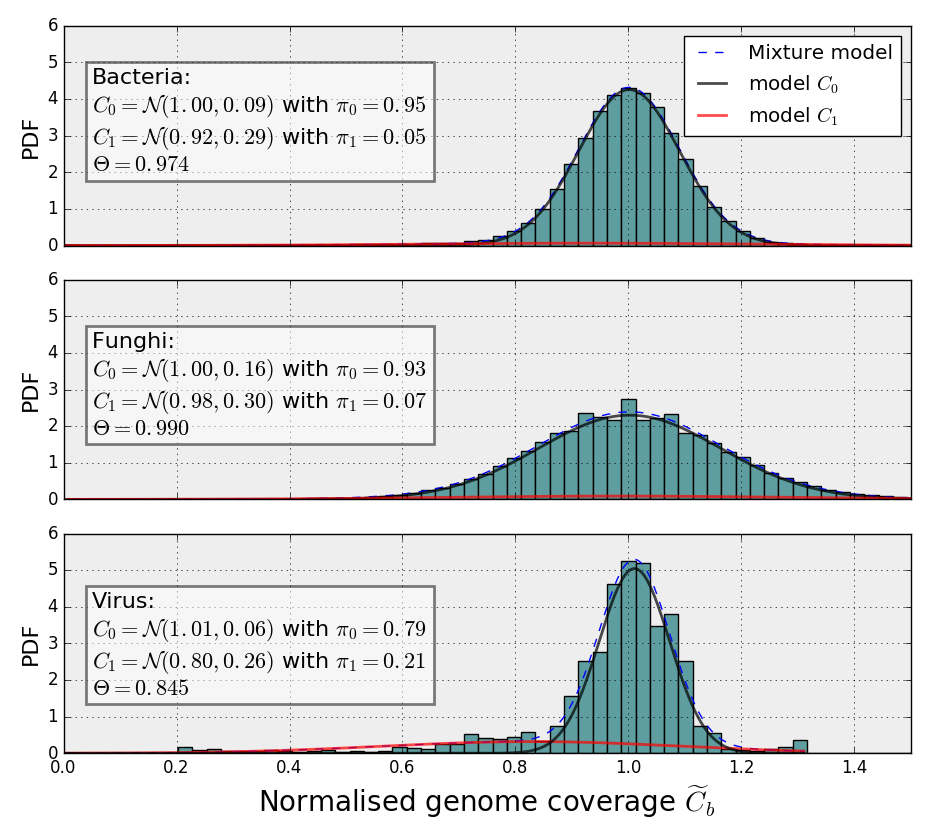
\includegraphics[height=0.9\textheight, 
    width=1\textwidth]{images/figure_em.png}
\end{center} 
\end{frame}



\begin{frame}
\frametitle{C. From a constant to adaptative $z$-score}

Assuming that the central distribution is the null hypothesis, 
we can now  assign a \textcolor{blue}{$z$-score in the normalised space}:

\begin{equation}
z(b) = \frac{\widetilde{C}(b)-\widetilde{\mu}_0}{\widetilde{\sigma}_0}
\nonumber
\end{equation}

We can  replace $\widetilde{C}_b$ by its expression  ($C_b / RM_W(b)$) and
express $C_b$ as a function of the running median, the $z(b)$ and the parameters 
of the central distribution:

\begin{equation}
C(b) = \left(  \widetilde{\mu}_0  + z(b) \widetilde{\sigma}_0  \right)RM_W(b).
\nonumber
\end{equation}

\end{frame}

%%%%%%%%%%%%%%%%%%%%%%%%%%%%%%%%%%%%%%%%%%%%%%
\begin{frame}
\frametitle{C. From a constant to adaptative $z$-score}
\begin{block}{}
We can now set a constant threshold in the normalised space (e.g. $\lambda \pm 3$) 
and get an adaptative threshold in the original space.
\end{block}

We can 
derive an \textcolor{blue}{adaptative threshold} in the 
original space that is function of the genome position: 

\begin{equation}
\tilde{\delta}^\pm(b) = \left( \widetilde{\mu}_0 \pm \lambda^\pm\times \widetilde{\sigma}_0    \right)RM_W(b).
\end{equation}

\end{frame}

\begin{frame}
 \frametitle{constant thresholds in the original space}
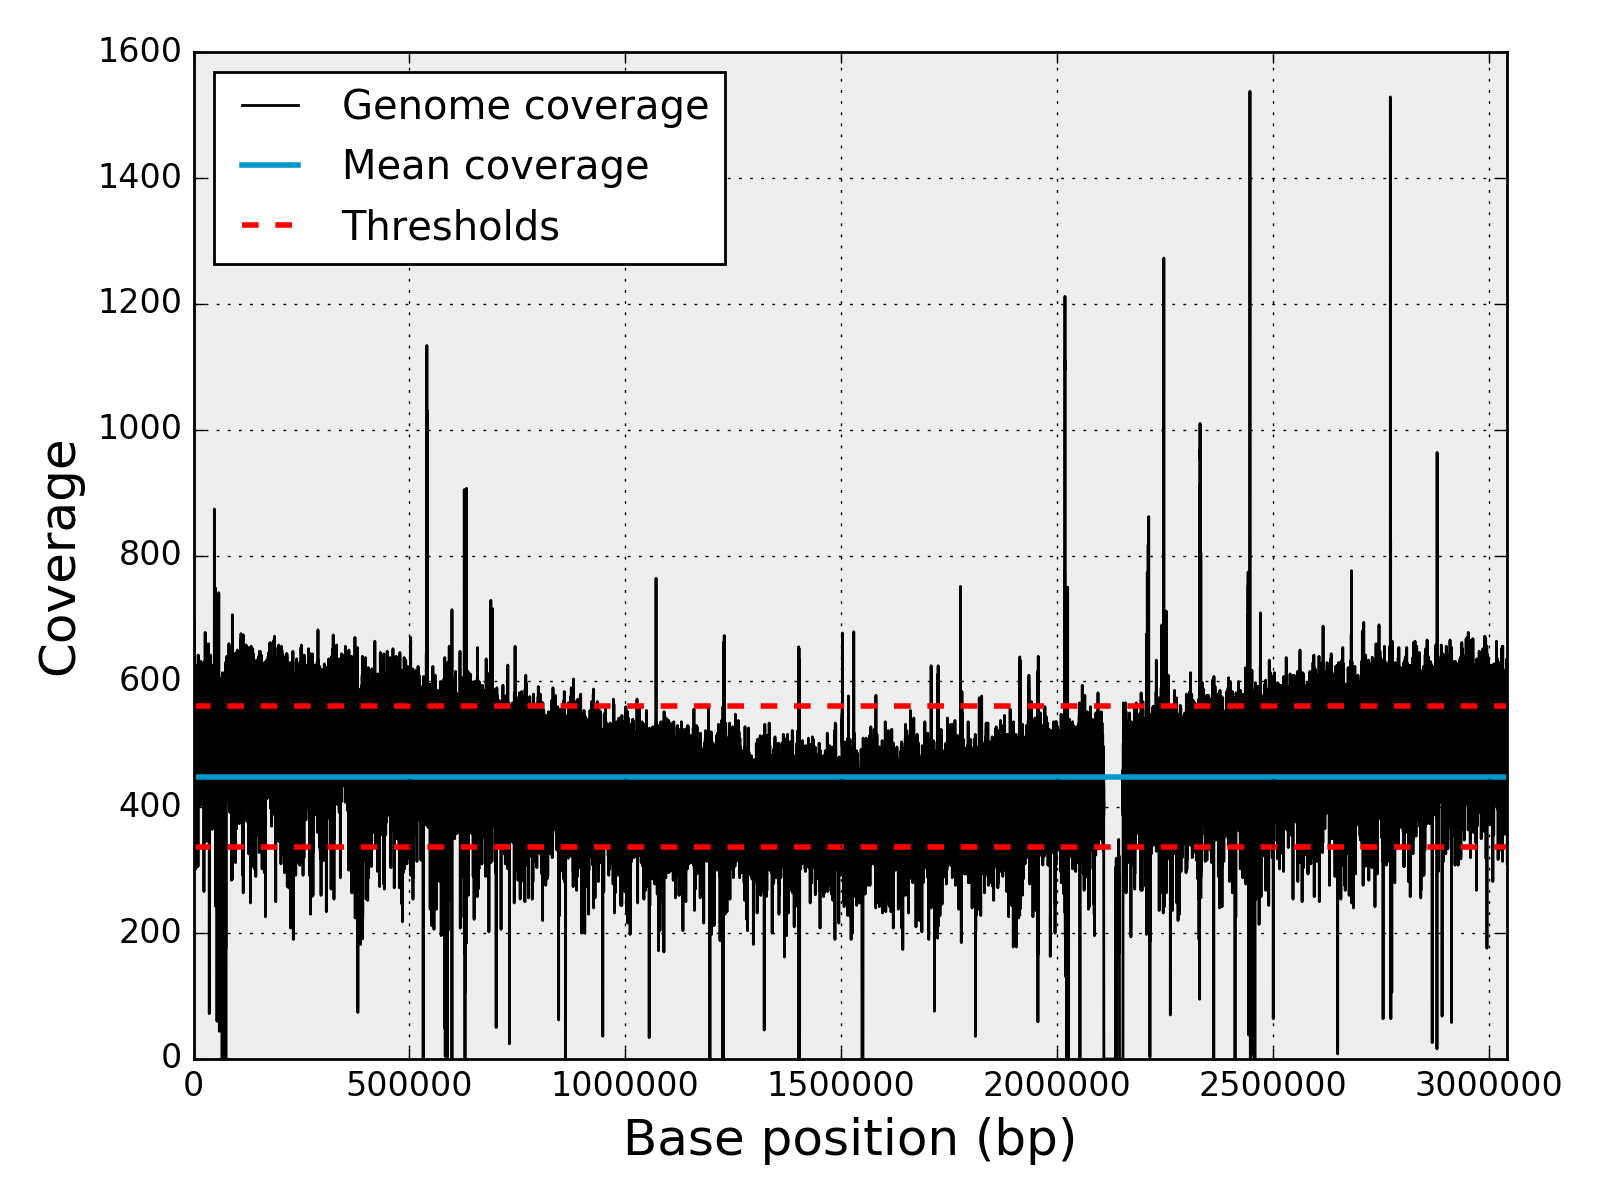
\includegraphics[height=0.9\textheight, 
    width=1\textwidth]{images/fig1.png}
 \end{frame}


 \begin{frame}
 \frametitle{constant thresholds in the normalised space}
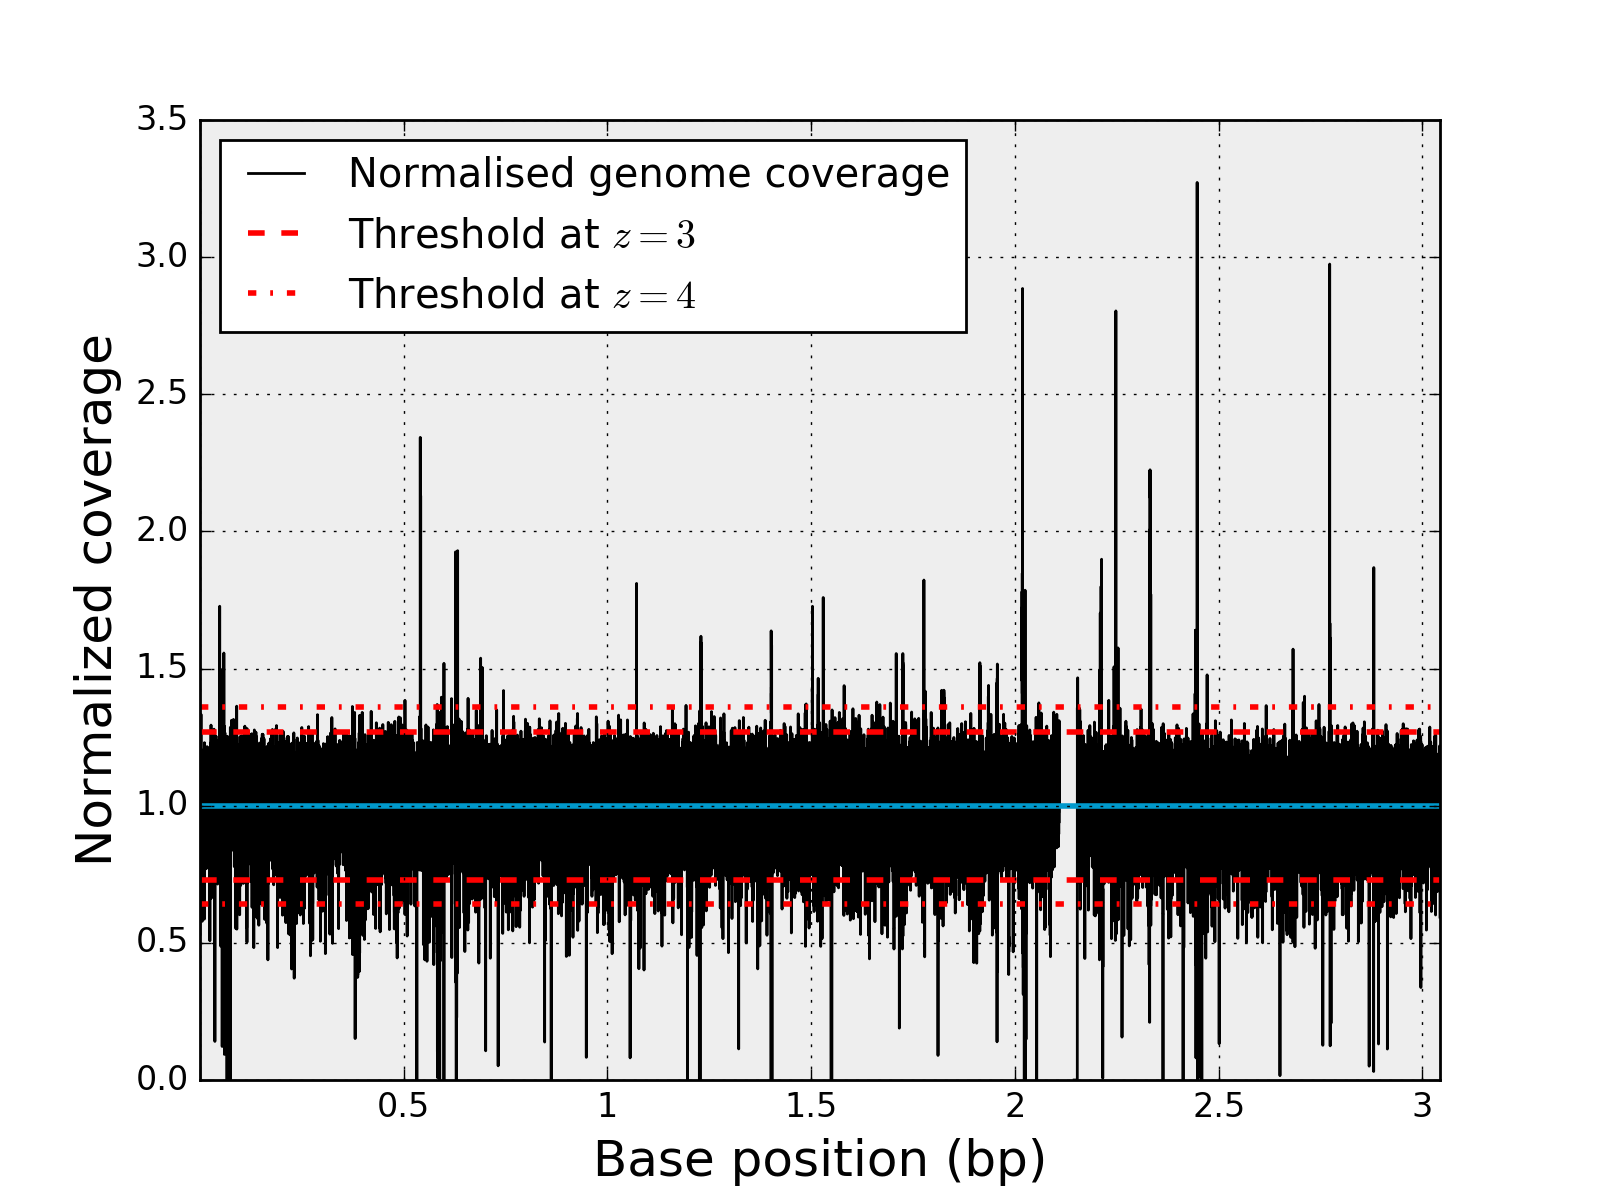
\includegraphics[height=0.9\textheight, 
    width=1\textwidth]{images/fig2.png}
\end{frame}

 
\begin{frame}
 \frametitle{adaptative thresholds in the original space}
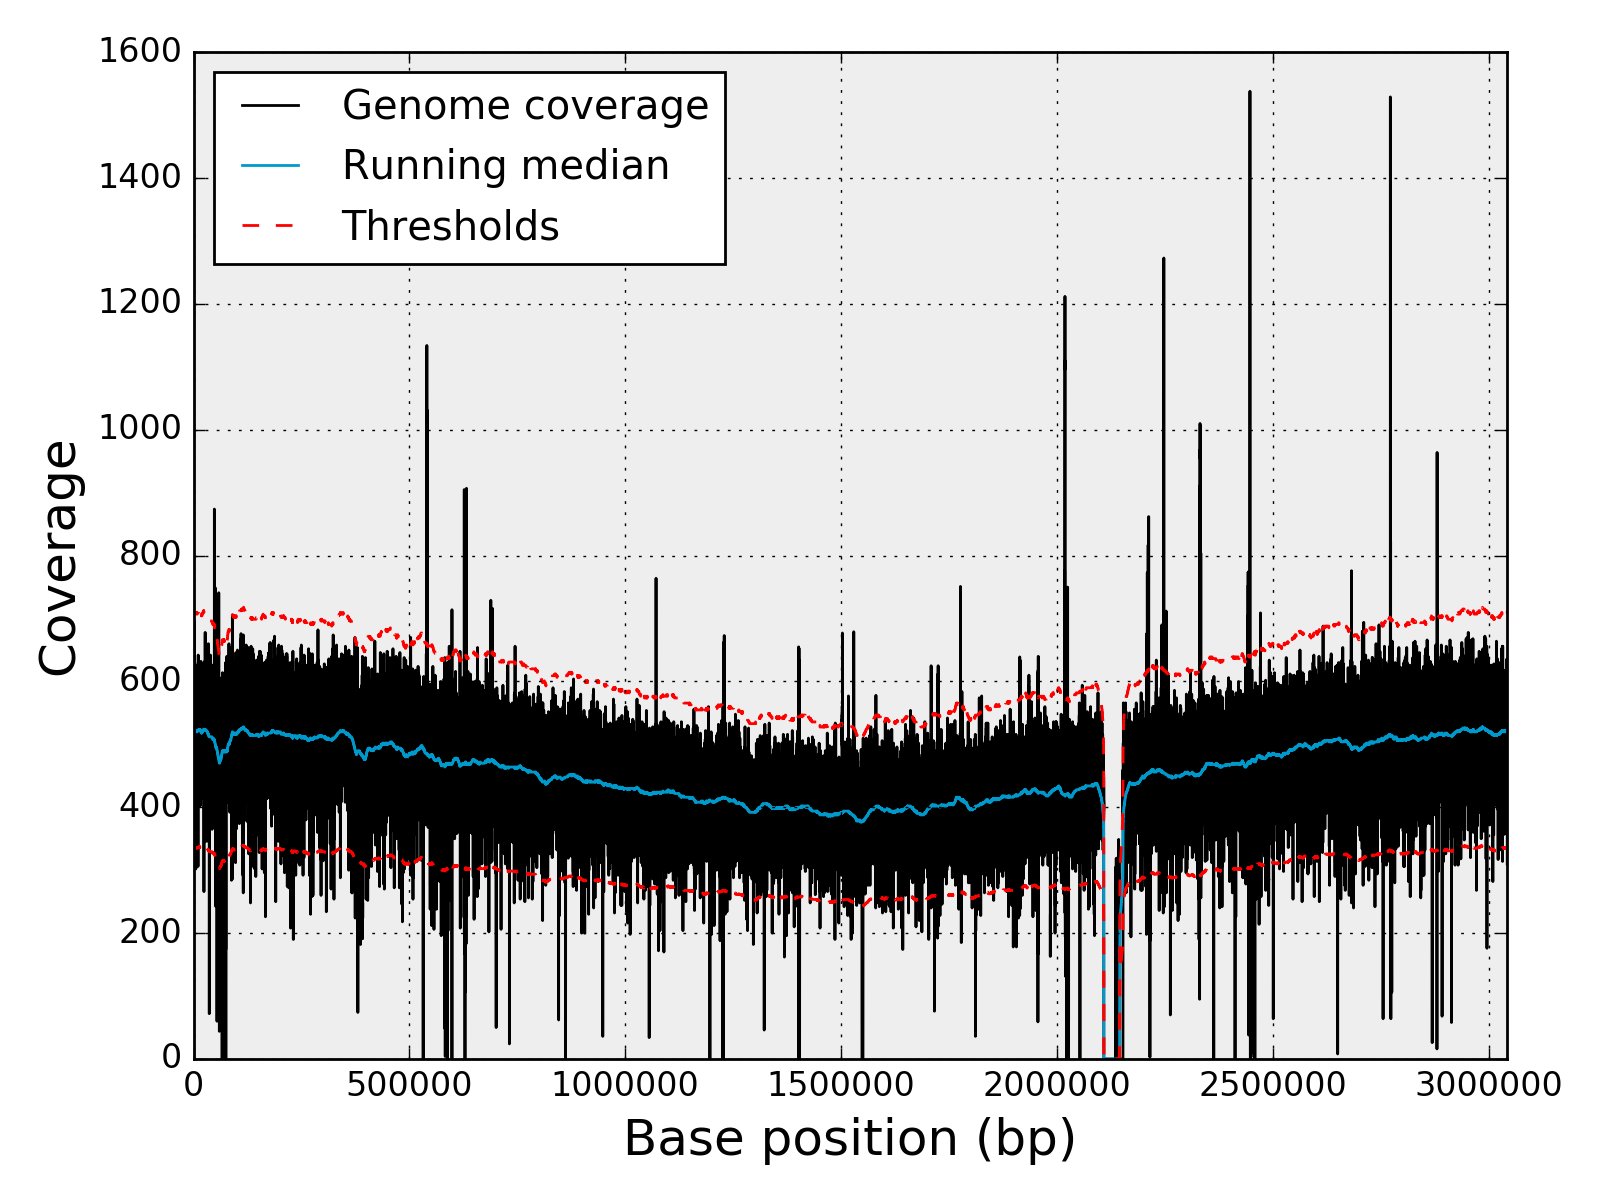
\includegraphics[height=0.9\textheight, 
    width=1\textwidth]{images/fig3.png}
\end{frame}

 
 
\begin{frame}
\frametitle{D. Regions of interest (clustering)}

\begin{block}{}
On a 3Mb genome with low thresholds the number of outliers are high. 
$\lambda=3$ means about 4000 events by pure chance.
\end{block}

\begin{block}{}
We need a strategy to reduce the number of interesting events. This is 
achieved by clustering the data.
\end{block}

\begin{block}{}
Besides, to cluster close-by events further, we proceed with a double-thresholds 
approach.
\end{block}
 
\end{frame}


\begin{frame}
 \frametitle{Double thresholds}
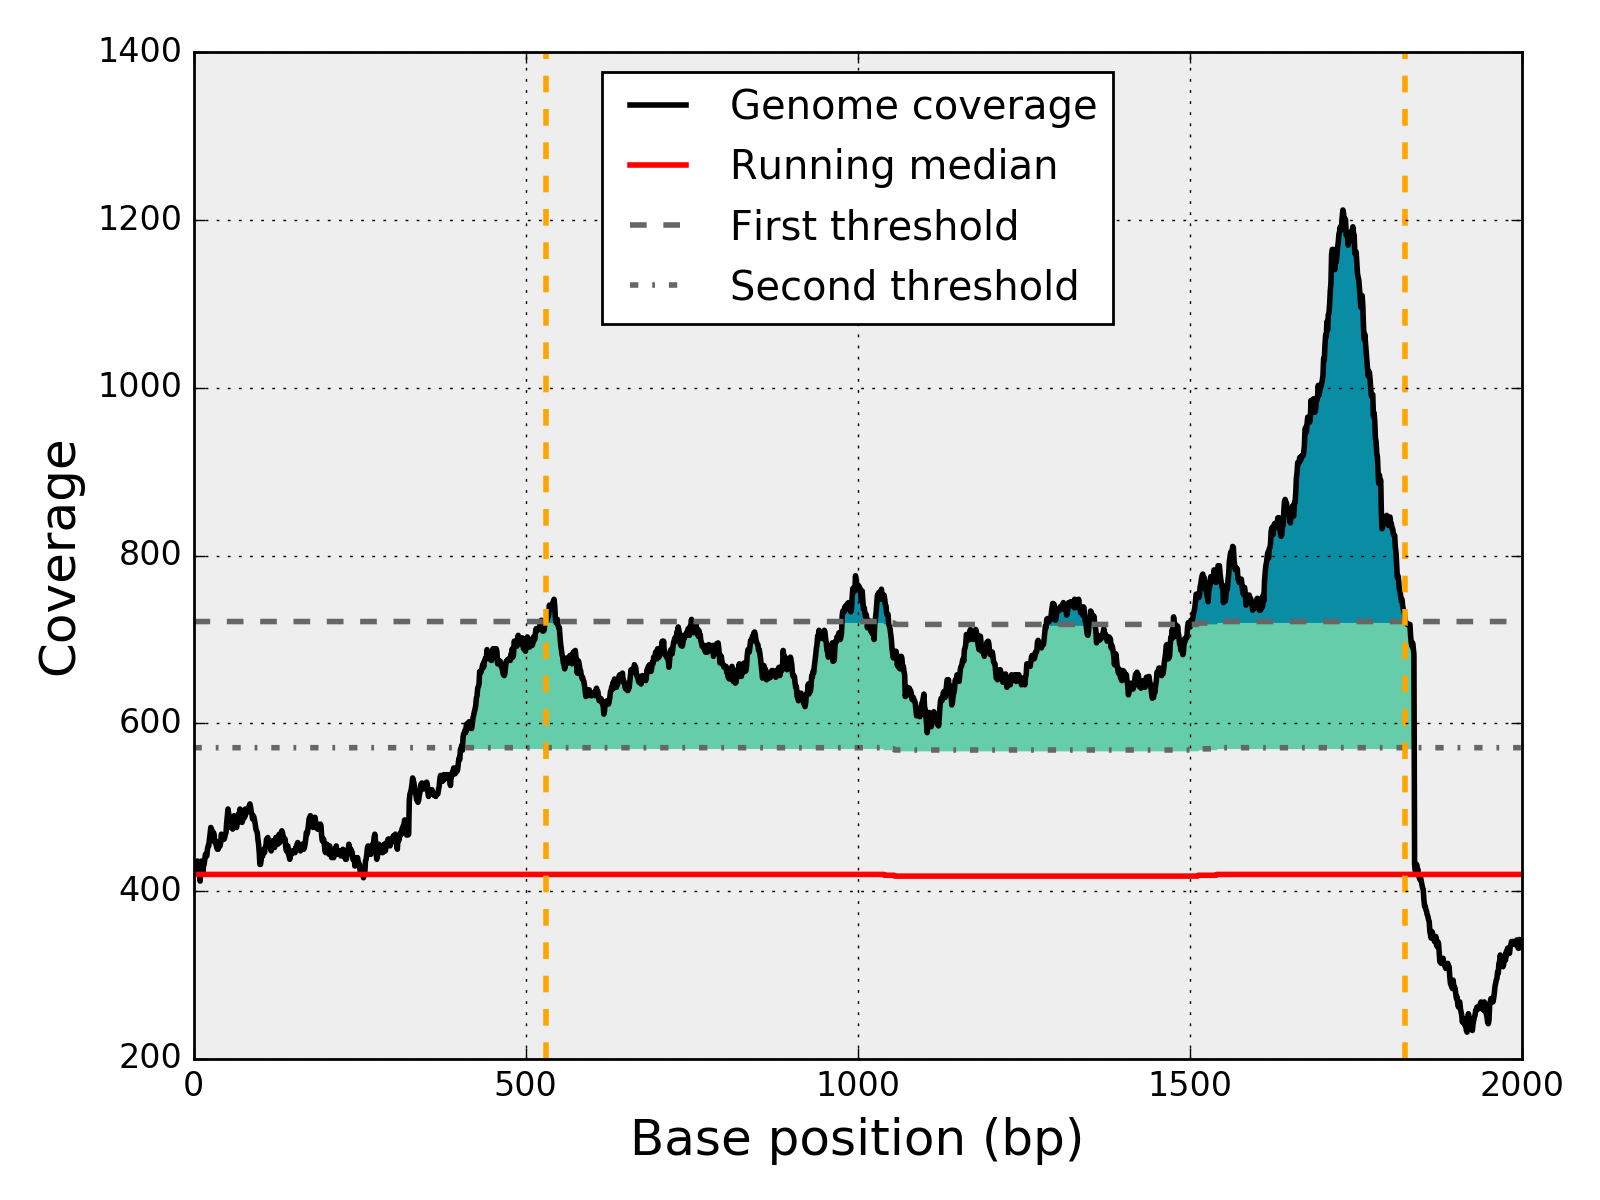
\includegraphics[height=0.9\textheight, 
    width=1\textwidth]{images/double_threshold.png}
\end{frame}

\begin{frame}[fragile]
\begin{lstlisting}{python}
sequana_coverage --download-genbank JB409847
sequana_coverage --input JB409847.bed -w 3001 --circular 
                 --genbank JB409847.gbk --show-html
\end{lstlisting}
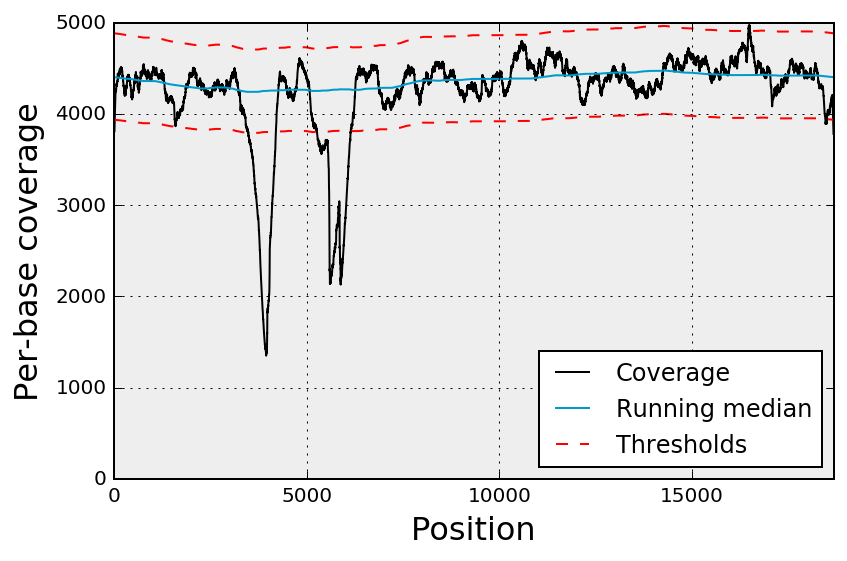
\includegraphics[height=0.7\textheight, 
    width=1\textwidth]{images/virus.png}
\end{frame}


\begin{frame}
 \frametitle{Summary}
 \begin{itemize}
    \item A robust and fast algo. to detect under/over covered regions.

    \item The algorithm is made of 3 steps:
    \begin{enumerate}
        \item Normalisation (running median)
        \item Set a statistics using EM to estimate mixture model
        \item Clustering of events in original space
    \end{enumerate}
    \item Implementation in Sequana as a standalone 
    \begin{itemize}
        \item HTML reports with ROIs provided as sortable tables
        \item Identify repeated regions
        \item A genbank can be provided to annotate the report
    \end{itemize}
\end{itemize}
  

 \footnotesize{
Dimitri Desvillechabrol, Christiane Bouchier, Sean Kennedy, Thomas Cokelaer
\textit{Detection and characterization of low and high genome coverage 
regions using an efficient running median and a double threshold approach.}
bioRxiv 092478; doi: http://dx.doi.org/10.1101/092478
}
\end{frame}



\end{document}
